\documentclass[tikz]{standalone}

\usepackage[latin1]{inputenc}
\usepackage{tikz}

% GNUPL
\begin{document}
\pagestyle{empty}


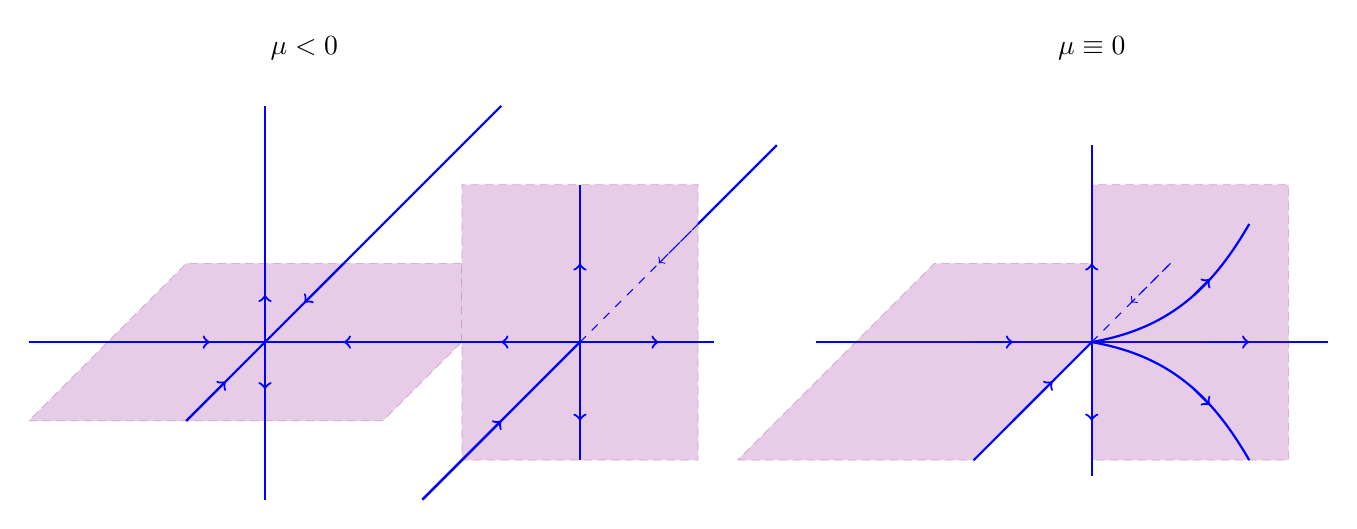
\begin{tikzpicture}
    %\mu<0
    \coordinate [label=-90:$\mu<0$] (8) at (3.5,7);
    \draw[violet, densely dashed][fill = violet, opacity=0.2]  (0,2) -- (4.5,2) -- (5.5,3) -- (5.5,1.5) -- (8.5,1.5) --(8.5,5) -- (5.5,5)--(5.5,4) --(2,4)--(0,2);
    \draw[violet, densely dashed][fill = violet, opacity=0.2]  (5.5,3) -- (5.5,4);
    \draw[blue,thick] (0,3) -- (8.7,3);
    \draw[blue,thick] [->] (2,3) -- (2.3,3);
    \draw[blue,thick] [<-] (4,3) -- (4.5,3);
    \draw[blue,thick] [->] (3,2.5) -- (3,2.4);
    \draw[blue,thick] [->] (3,3.5) -- (3,3.6);
    \draw[blue,thick] [->] (2,2) -- (2.5,2.5);
    \draw[blue,thick] [->] (4,4) -- (3.5,3.5);
	\draw[blue,thick] (3,1) -- (3,6);
	\draw[blue,thick] (2,2) -- (6,6);
	\draw[blue,thick] (7,1.5) -- (7,5);
    \draw[blue,thick] [->] (7,2.5) -- (7,2);
    \draw[blue,thick] [->] (7,3) -- (7,4);
    \draw[blue,thick] [->] (7,3) -- (6,3);
    \draw[blue,thick] [->] (7,3) -- (8,3);
    \draw[blue,thick] (5,1) -- (7,3);
    \draw[blue,thick] [->] (5,1) -- (6,2);
    \draw[blue,thick] (9.5,5.5) -- (8.5,4.5);
    \draw[blue,dashed] (7,3) -- (8.5,4.5);
    \draw[blue,dashed] [->] (8.5,4.5) -- (8,4);

	% %\mu=0
	\coordinate [label=-90:$\mu \equiv0$] (8) at (13.5,7);

     \draw[blue,thick] (10,3) -- (16.5,3);
     \draw[violet, densely dashed][fill = violet, opacity=0.2]  (9,1.5) -- (12,1.5) -- (13.5,3) -- (13.5,1.5) -- (16,1.5) --(16,5) -- (13.5,5)--(13.5,4) --(11.5,4)--(9,1.5);
     \draw[violet, densely dashed][fill = violet, opacity=0.2]  (13.5,3) -- (13.5,4);
     \draw[blue,thick] (13.5,1.3) -- (13.5,5.5);
     \draw[blue,thick] (12,1.5) -- (13.5,3);
     \draw[blue,thick] (13.5,3) to [out=10,in=-120] (15.5,4.5);
     \draw[blue,thick] (13.5,3) to [out=-10,in=120] (15.5,1.5);
     \draw[blue,dashed] (13.5,3) -- (14.5,4);
     \draw[blue,thick] [->] (12,3) -- (12.5,3);
     \draw[blue,thick] [->] (15,3) -- (15.5,3);
     \draw[blue,thick] [->] (13.5,3) -- (13.5,4);
     \draw[blue,thick] [->] (13.5,3) -- (13.5,2);
     \draw[blue,thick] [->] (12.5,2) -- (13,2.5);
     \draw[blue,dashed] [->] (14.5,4) -- (14,3.5);
     \draw[blue,thick] [->] (14.8,3.6) -- (15,3.8);
     \draw[blue,thick] [->] (14.8,2.4) -- (15,2.2);
 %    \draw[semithick] [->] (8,3) -- (9,3);
 %    \draw[semithick] [->] (11.5,3) -- (12,3);
 %    \draw[teal,densely dashed][fill = teal, opacity=0.2] (9.5,0.5) -- (11.5,2.5) -- (11.5,6.5) -- (9.5,4.5) -- (9.5,0.5);
 %    \draw [red,thick] (11,2) to [out=180,in=-90] (9.8,3) to [out=90,in=180] (10.5,4) to [out=0,in=90] (11,3) to [out=-90,in=0] (10.5,2.6) to [out=180,in=-90] (10.2,3) to [out=90,in=180] (10.5,3.2);
 %    \draw [red,thick] [->] (10.5,4) --(10.51,4);
 %    \draw [red,thick] (8,4.5) to [out=30,in=90] (9,3) to [out=-90,in=0] (8.5,2.3) to [out=180,in=-90] (8.2,3) to [out=90,in=180] (9.1,3.7) to [out=0,in=20] (9.25,2.8);
 %    \draw [red,thick] [->] (8.4,4.54) --(8.41,4.54);
 %    \draw [red,thick] (11.5,4.5) to [out=-30,in=0] (11.8,2.3) to [out=-180,in=180] (11.9,3.5) to [out=0,in=0] (12.5,2.5) to [out=180,in=180] (12.8,3.3);
 %    \draw [red,thick] [->] (11.7,4.35) --(11.72,4.34);
 %    \draw [fill] (10.5,3) circle [radius=0.05];

 %    %\mu>0
 %    \coordinate [label=-90:$\mu>0$] (8) at (16.5,9);

 %    \draw[semithick] [->] (14,8) -- (19,8) node[right] {$U_1$};
 %    \draw[semithick] [->] (16,8) -- (17,8);


 %    \draw[semithick] [->] (14,3) -- (19,3) node[above] {$U_1$};
 %    \draw[semithick] [->] (15,3) -- (16,3);
 %    \draw [red,thick] (14,4.5) to [out=30,in=0] (15,2) to [out=180,in=180] (16,3.8) to [out=0,in=0] (16.5,2.5) to [out=180,in=180] (17.2,3.5) to [out=0,in=0] (17.8,2.6) to [out=180,in=180] (18.4,3.2); 
 %    \draw [red,thick] [->] (14.5,4.5) --(14.51,4.495);
\end{tikzpicture}


\end{document}